%%%%%%%%%%%%%%%%%%%%%%%%%%%%%%%%%%%%

\section{Evaluating the normal approximation}

%%%%%%%%%%%%%%%%%%%%%%%%%%%%%%%%%%%%

\subsection{Normal probability plot}

%%%%%%%%%%%%%%%%%%%%%%%%%%%%%%%%%%%%

\begin{frame}
\frametitle{Normal probability plot}

A histogram and \hl{normal probability plot} of a sample of 100 male heights.

\begin{center}
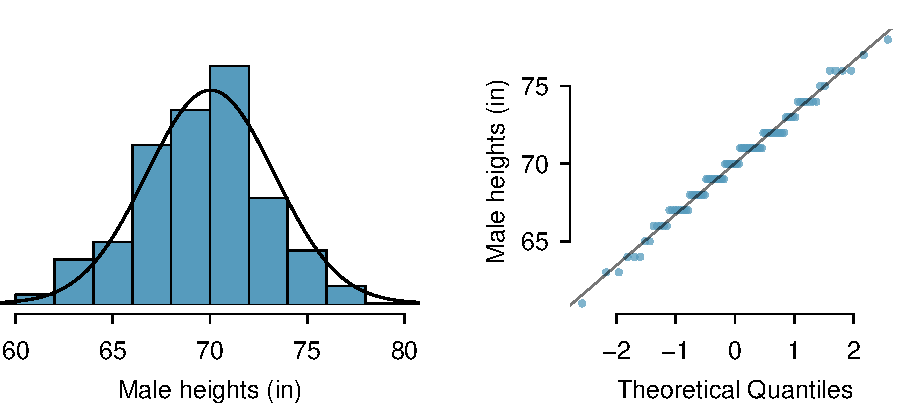
\includegraphics[width=0.9\textwidth]{4-2_evaluating_normal_approx/figures/fcidMHeights/fcidMHeights}
\end{center}

\end{frame}

%%%%%%%%%%%%%%%%%%%%%%%%%%%%%%%%%%%%

\begin{frame}
\frametitle{Anatomy of a normal probability plot}

\begin{itemize}

\item Data are plotted on the y-axis of a normal probability plot, and theoretical quantiles (following a normal distribution) on the x-axis.

\item If there is a linear relationship in the plot, then the data follow a nearly normal distribution.

\item Constructing a normal probability plot requires calculating percentiles and corresponding z-scores for each observation, which is tedious. Therefore we generally rely on software when making these plots.

\end{itemize}

\end{frame}

%%%%%%%%%%%%%%%%%%%%%%%%%%%%%%%%%%%%

\begin{frame}

\dq{Below is a histogram and normal probability plot for the NBA heights from the 2008-2009 season. Do these data appear to follow a normal distribution?}

\begin{center}
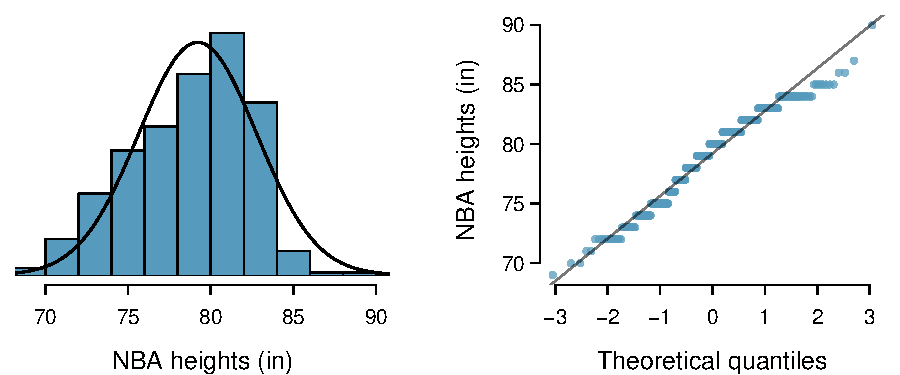
\includegraphics[width=0.8\textwidth]{4-2_evaluating_normal_approx/figures/nbaNormal/nbaNormal}
\end{center}

\pause

\dq{Why do the points on the normal probability have jumps?}

\end{frame}

%%%%%%%%%%%%%%%%%%%%%%%%%%%%%%%%%%%%

\begin{frame}
\frametitle{Normal probability plot and skewness}

\twocol{0.2}{0.8}{
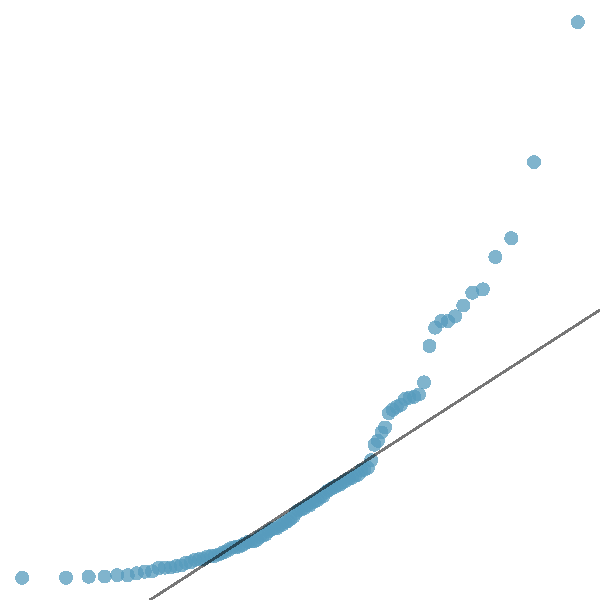
\includegraphics[width=0.8\textwidth]{4-2_evaluating_normal_approx/figures/skew/qq_rs}
}
{
Right skew - Points bend up and to the left of the line.
}

\twocol{0.2}{0.8}{
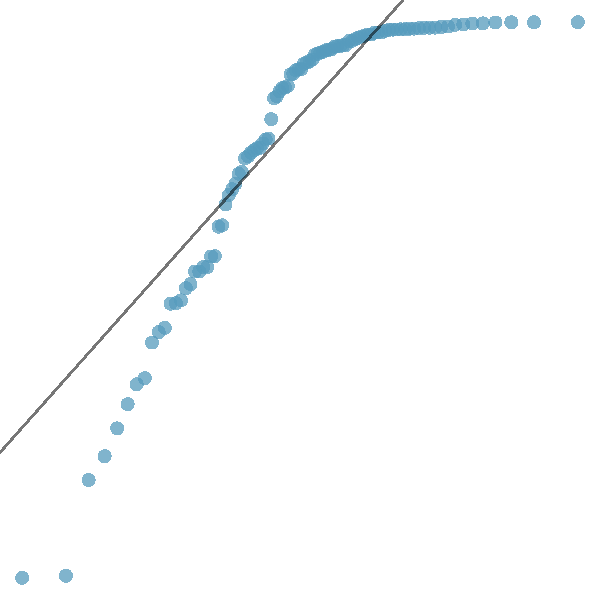
\includegraphics[width=0.8\textwidth]{4-2_evaluating_normal_approx/figures/skew/qq_ls}
}
{
Left skew- Points bend down and to the right of the line.
}

\twocol{0.2}{0.8}{
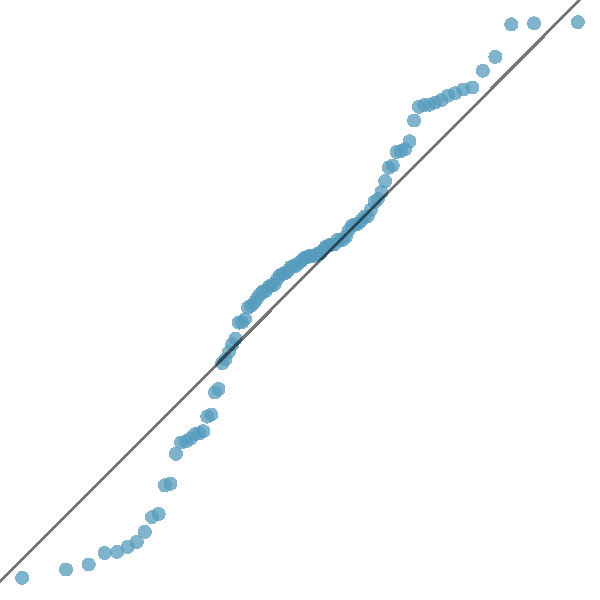
\includegraphics[width=0.8\textwidth]{4-2_evaluating_normal_approx/figures/skew/qq_st}
}
{
Short tails (narrower than the normal distribution) - Points follow an S shaped-curve.
}

\twocol{0.2}{0.8}{
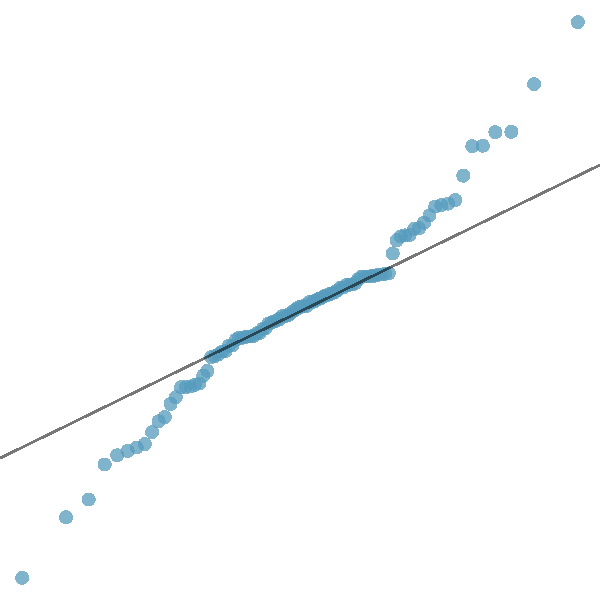
\includegraphics[width=0.8\textwidth]{4-2_evaluating_normal_approx/figures/skew/qq_lt}
}
{
Long tails (wider than the normal distribution) - Points start below the line, bend to follow it, and end above it.
}

\end{frame}

%%%%%%%%%%%%%%%%%%%%%%%%%%%%%%%%%%%%